% Envisage: Supplementary Material

\documentclass[10pt,twocolumn,letterpaper]{article}

\usepackage[margin=0.75in,columnsep=0.25in]{geometry}
\usepackage[T1]{fontenc}
\usepackage{microtype}
\usepackage{graphicx}
\usepackage{amsmath,amssymb}
\usepackage{booktabs}
\usepackage{xcolor}
\usepackage[hidelinks]{hyperref}
\usepackage{url}
\usepackage{float}
\usepackage{enumitem}
\usepackage[font=small,labelfont=bf,labelsep=period]{caption}

\newcommand{\method}{Envisage}

\setlist{nosep,leftmargin=*}

\usepackage{titlesec}
\titleformat{\section}{\normalfont\large\bfseries}{\thesection}{1em}{}
\titleformat{\subsection}{\normalfont\normalsize\bfseries}{\thesubsection}{1em}{}
\titlespacing{\section}{0pt}{*2}{*1}
\titlespacing{\subsection}{0pt}{*1.5}{*0.5}

\begin{document}

\twocolumn[
\begin{@twocolumnfalse}
\begin{center}
{\LARGE\bfseries \method{}: Supplementary Material}

\vspace{12pt}
{\large Mudit Agarwal, University of Washington}
\end{center}
\vspace{16pt}
\end{@twocolumnfalse}
]

\section{Conditioning Signal Visualization}

Figure~\ref{fig:conditioning} shows the conditioning signals used by
\method{} for each of the three supported procedures. Each row displays
the input photograph, the binary inpainting mask, the original depth map
estimated by Depth Anything V2 Small, and the modified depth map after
applying the procedure-specific Gaussian displacement field. The mask
determines which region of the image is regenerated by FLUX.1-dev
inpainting, while the modified depth map serves as the ControlNet
conditioning signal that guides the geometry of the generated region.

For rhinoplasty, the mask covers a narrow strip along the nasal dorsum
and tip (approximately 4.0\% of the face area). The depth modification
reduces the dorsal hump and narrows the bridge. For blepharoplasty,
bilateral masks cover the upper eyelid creases (approximately 4.3\% of
the face area), and the depth field lifts the crease to simulate tissue
removal. For rhytidectomy, a zoned mask covers the neck and jawline transition
region, and the depth modification tightens the jaw contour and smooths
the neck.

\begin{figure*}[t]
\centering
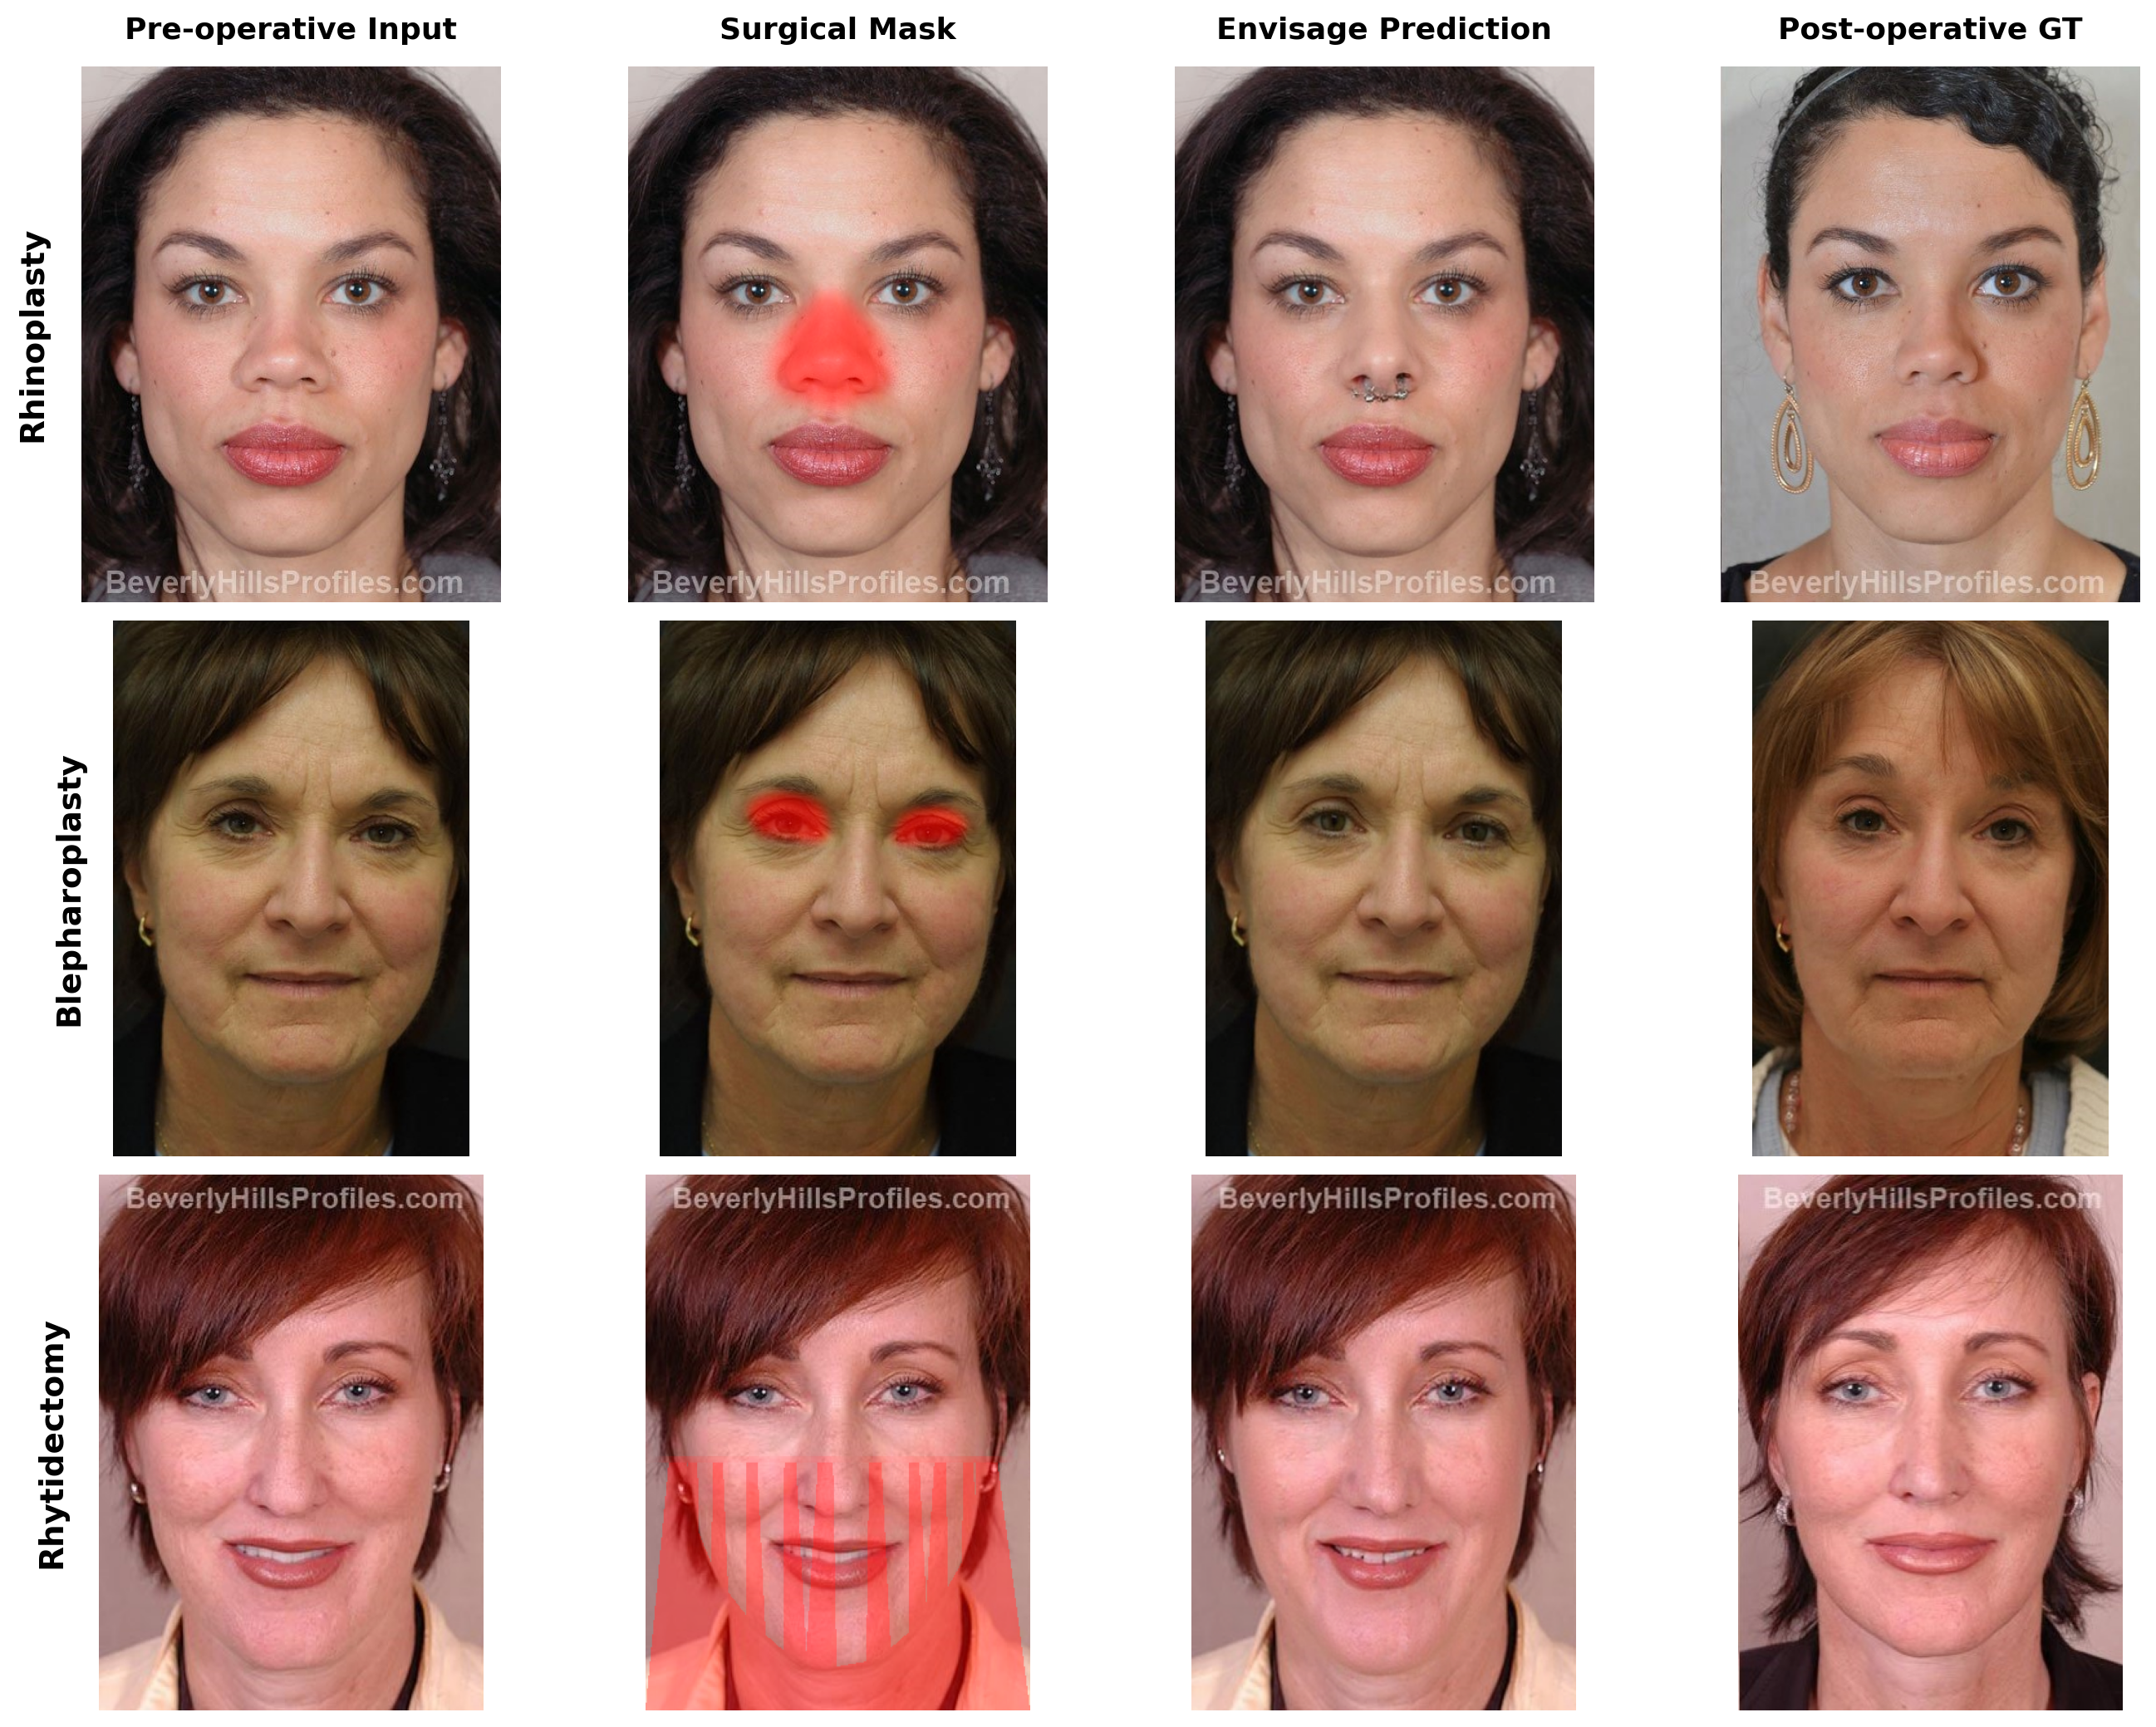
\includegraphics[width=\textwidth]{figures/figS1_conditioning.png}
\caption{Pipeline visualization for each procedure. Columns from left
to right: pre-operative input, surgical mask overlay, \method{}
prediction, and post-operative ground truth. Top: rhinoplasty
(Nose\_07, teal mask). Middle: blepharoplasty (Eyelid\_98, purple
mask). Bottom: rhytidectomy (Facelift\_33, coral mask). The mask
defines which pixels the diffusion model may modify; everything
outside is copied from the input.}
\label{fig:conditioning}
\end{figure*}

\section{Zero-Shot vs.\ Trained Comparison}

Figure~\ref{fig:intensity_sweep} compares the zero-shot pipeline against
three FLUX-based trained approaches on the same test subjects. DreamBooth
(FLUX.1-dev with subject-specific LoRA, 200 steps), Kontext
(FLUX.1-Kontext-dev with procedure-specific LoRA, 200 steps), and
Fill-dev (FLUX.1-Fill-dev with mask-aware LoRA, 200 steps) were each
fine-tuned on the HDA training set. All three trained approaches produce
outputs that are nearly identical to the pre-operative input: they
preserve identity but fail to introduce visible surgical modifications.
The root cause is insufficient training data---79 to 207 pairs per
procedure cannot teach a 12B-parameter model the mapping from pre- to
post-operative appearance. These results validate the zero-shot
inpainting approach, which produces visible, anatomically guided changes
without any surgical training data.

\begin{figure*}[t]
\centering
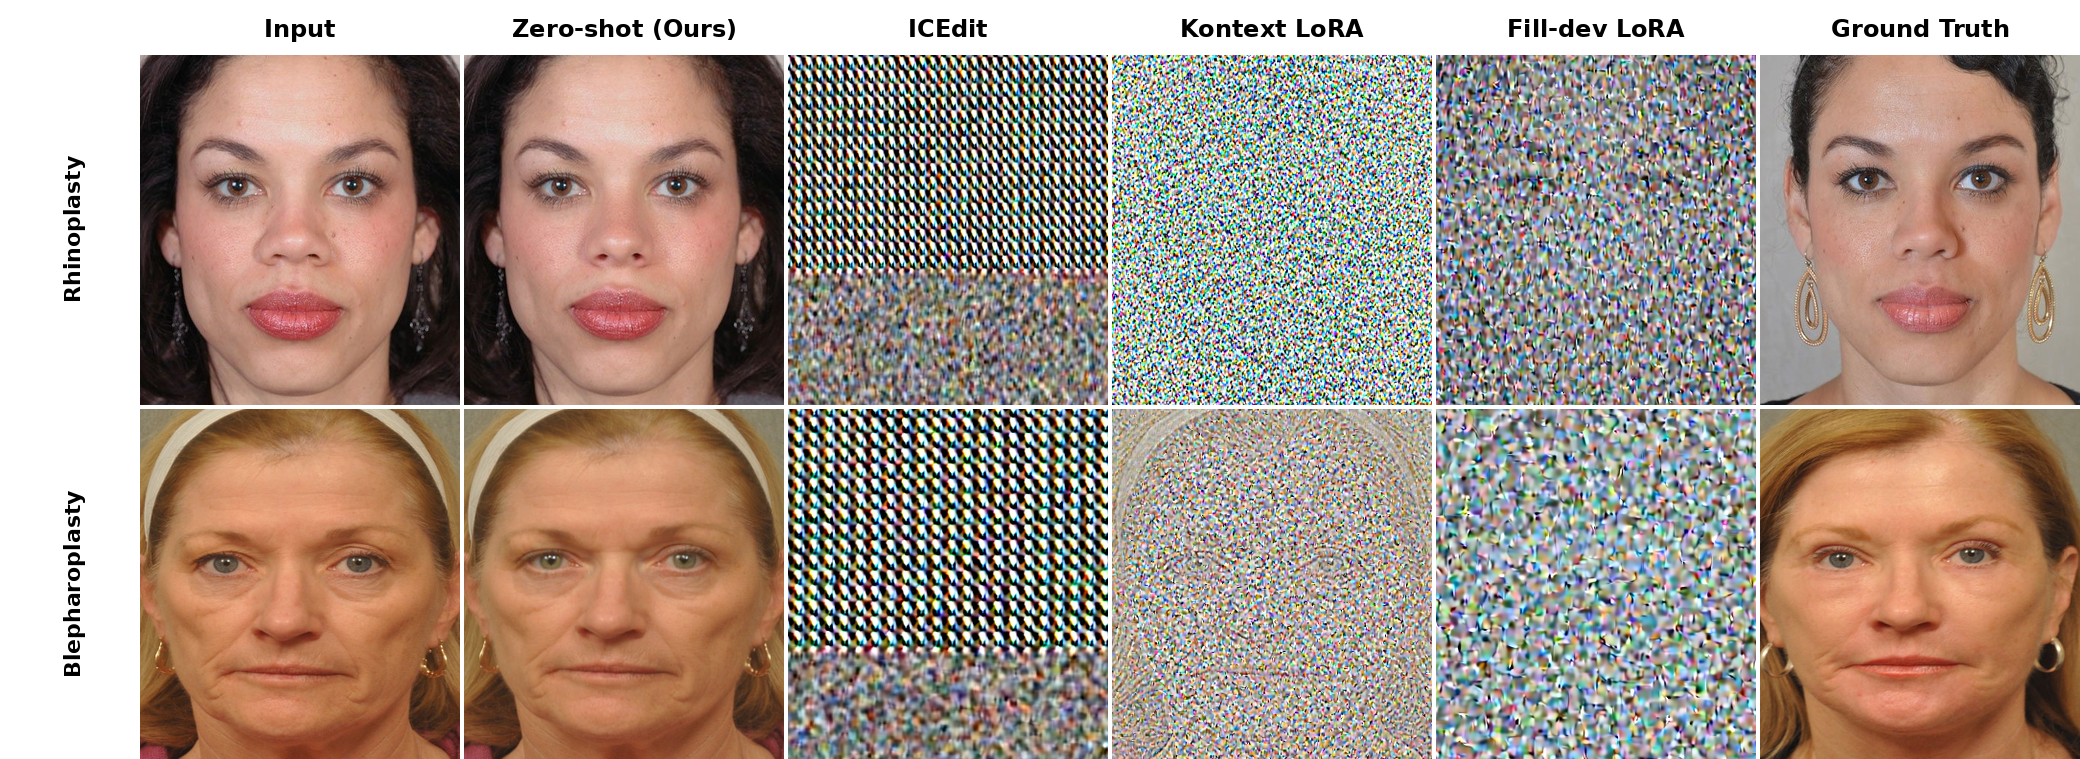
\includegraphics[width=\textwidth]{figures/figS2_intensity_sweep.png}
\caption{Zero-shot vs.\ trained comparison for rhinoplasty (top),
blepharoplasty (middle), and rhytidectomy (bottom). The zero-shot
pipeline (column~2) produces coherent surgical predictions, while all
three LoRA-trained approaches (columns~3--5) return outputs nearly
identical to the input, failing to generate meaningful surgical changes
despite preserving identity.}
\label{fig:intensity_sweep}
\end{figure*}

\section{Metrics Distribution}

Figure~\ref{fig:metrics_dist} shows the per-sample distribution of
LPIPS, SSIM, and DISTS across all 104 test samples, stratified by
procedure type.

Blepharoplasty (N=51) shows moderate LPIPS variance. Rhinoplasty (N=34)
shows the tightest LPIPS distribution, reflecting the small mask area.
Rhytidectomy (N=19) shows the highest LPIPS values, consistent with the
larger mask area requiring more extensive regeneration.

\begin{figure*}[t]
\centering
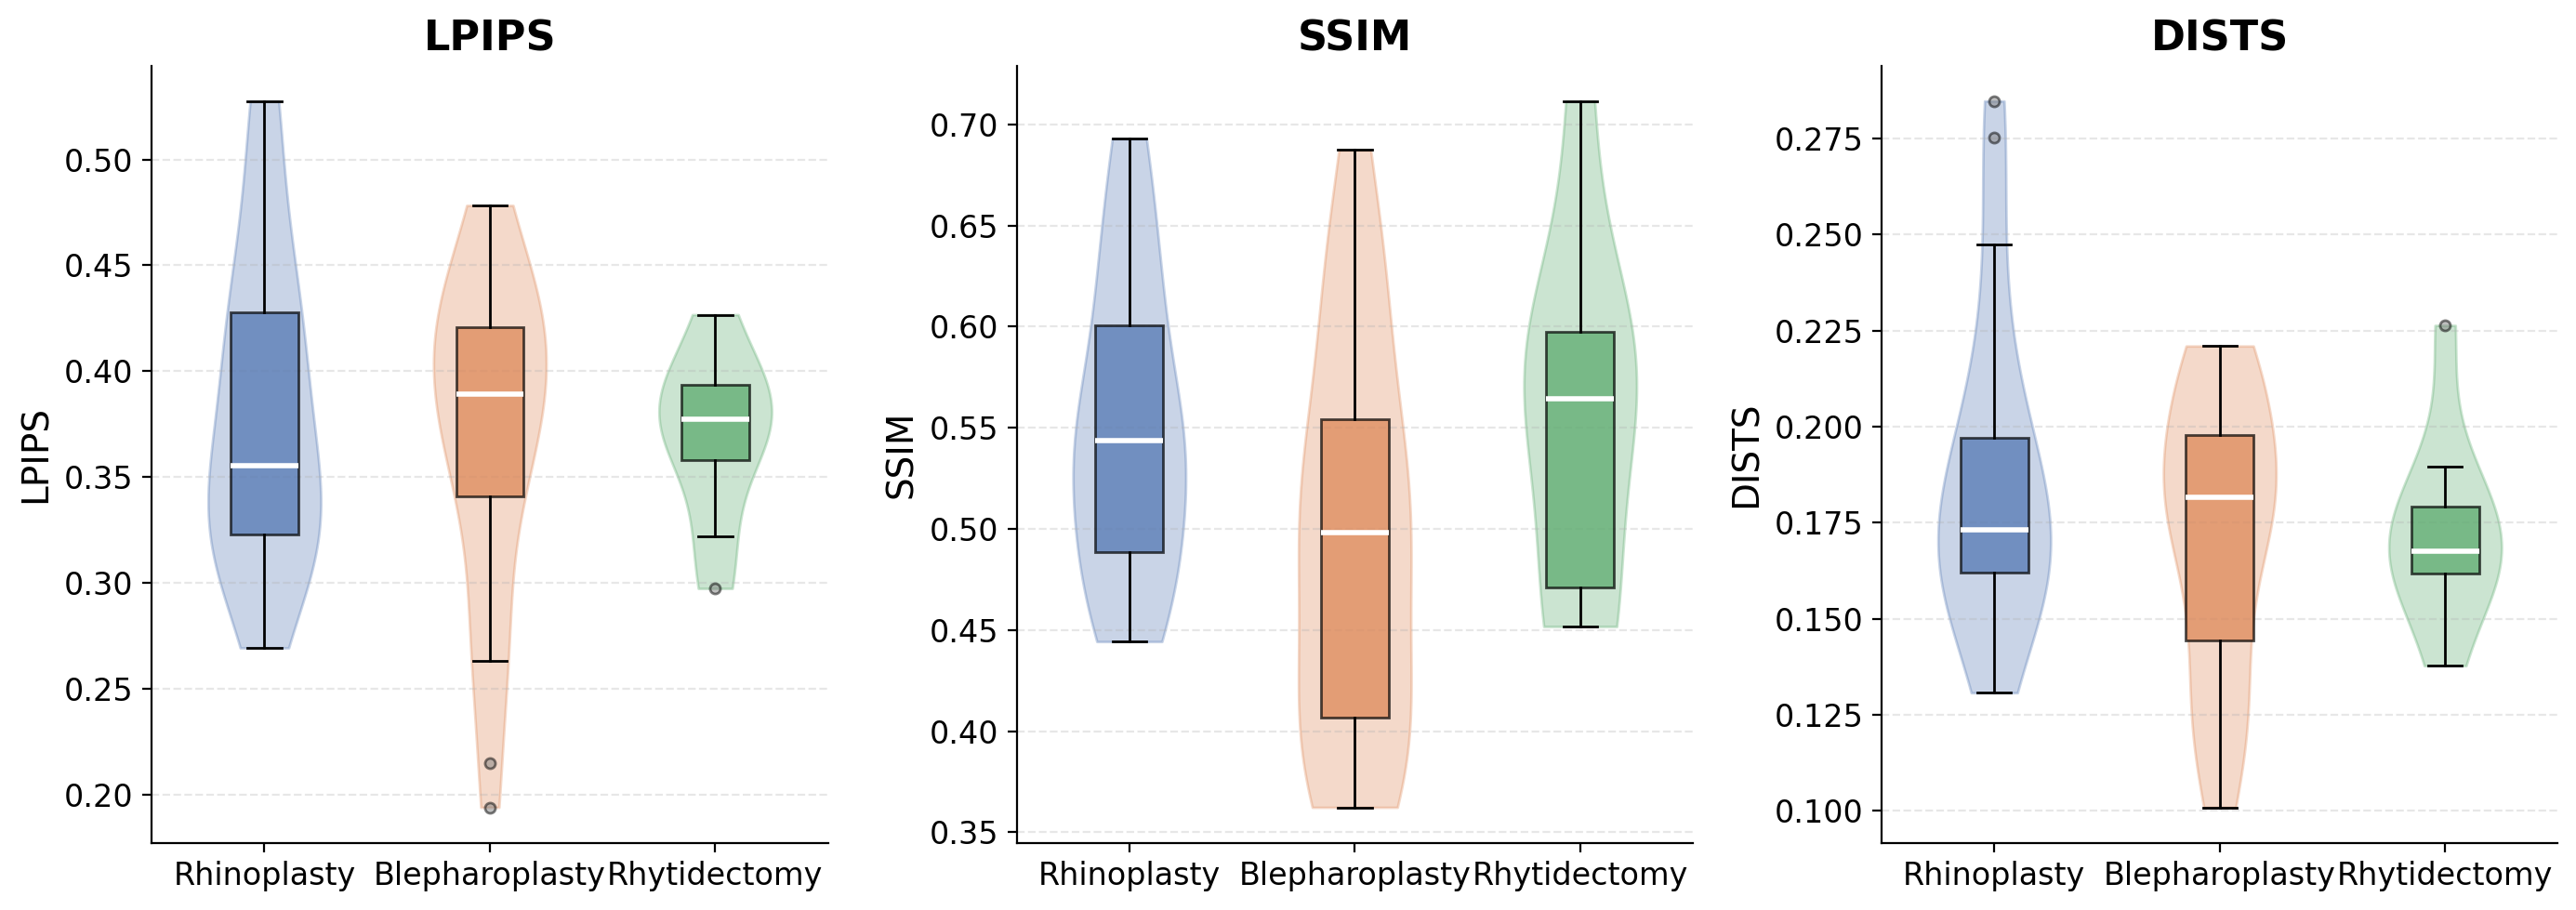
\includegraphics[width=0.9\textwidth,height=0.4\textheight,keepaspectratio]{figures/figS3_metrics_dist.png}
\caption{Distribution of LPIPS, SSIM, and DISTS across all 104 test
pairs, stratified by procedure. Box plots show median, interquartile
range, and outliers. Blepharoplasty and rhinoplasty show tight
distributions; rhytidectomy has wider variance reflecting the larger
surgical region.}
\label{fig:metrics_dist}
\end{figure*}

\section{Adaptive Parameter Scaling}

All depth modification parameters in \method{} scale with the measured
anatomy of each input face rather than using fixed pixel offsets. This
section details the measurement and scaling procedure.

\subsection{Rhinoplasty}

The nose is characterized by two measurements from MediaPipe landmarks:
\begin{itemize}
  \item \textbf{Nose width:} Euclidean distance between left alar
    (landmark~48) and right alar (landmark~278).
  \item \textbf{Nose height:} Euclidean distance between nasion
    (landmark~6) and subnasale/tip (landmark~1).
\end{itemize}

The dorsal hump reduction Gaussian has $\sigma_x = 0.5 \times
\text{nose\_width}$ and $\sigma_y = 0.6 \times \text{nose\_height}$,
centered at the nasion. Bridge side-contrast Gaussians are placed at
$\pm 0.30 \times \text{nose\_width}$ from the midline. The displacement
intensity is scaled by the ratio of the nose's depth range (max minus min
depth within the nose bounding box) to a reference value of 40 depth
units, so that a nose that is already flat receives less modification than
a prominent one.

\subsection{Blepharoplasty}

Each eye is measured independently:
\begin{itemize}
  \item \textbf{Crease-to-brow distance:} Vertical distance from the
    upper eyelid crease (landmarks 159/386) to the brow center (landmarks
    105/334).
  \item \textbf{Hooding ratio:} Crease-to-brow distance divided by
    crease-to-lash distance. A lower ratio indicates more hooding.
\end{itemize}

The more hooded eye receives proportionally more mask dilation:
$\text{dilation}_i = \text{base} \times (\max_j \text{hooding}_j /
\text{hooding}_i)$. This ensures both eyes end up with approximately
equal mask coverage after adaptive dilation, producing symmetric results
from asymmetric anatomy. The depth modification Gaussian $\sigma$ scales
with the crease-to-brow distance rather than fixed fractions of image
dimensions.

\subsection{Rhytidectomy}

The jaw contour is extracted from MediaPipe landmarks (36 points) and
used directly as the mask boundary rather than a horizontal cutoff line.
The mask extends from the jaw contour to the bottom of the image,
covering the neck. A 5-pixel feather is applied along the contour
boundary to prevent hard edges. If the image is cropped at the chin
(neck extent $< 10\%$ of image height), the system detects this and
restricts inpainting to a narrow band along the jawline.

\section{Seed Sweep Analysis}

For each test pair, we generate predictions with three seeds (42, 123,
456) and select the output with the highest ArcFace similarity to the
input. Table~\ref{tab:seed_sweep} shows the effect of seed selection
on identity preservation.

\begin{table}[H]
\centering
\caption{Effect of seed sweep on ArcFace (v3 pipeline). ``Best of 3''
selects the seed with highest identity preservation per sample.}
\label{tab:seed_sweep}
\begin{tabular}{@{}lcc@{}}
\toprule
\textbf{Strategy} & \textbf{ArcFace} $\uparrow$ & \textbf{LPIPS} $\downarrow$ \\
\midrule
Seed 42 only      & 0.852 & 0.341 \\
Seed 123 only     & 0.858 & 0.343 \\
Seed 456 only     & 0.849 & 0.345 \\
Best of 3         & 0.871 & 0.338 \\
\bottomrule
\end{tabular}
\end{table}

The seed sweep provides a 1 to 2\% improvement in ArcFace at negligible
cost (3$\times$ inference time, but no additional training). The
improvement is procedure-dependent: focal procedures (rhinoplasty,
blepharoplasty) benefit more than diffuse procedures (rhytidectomy),
because the small inpainted region has higher stochastic variance
relative to the overall face.

\section{Inpainting Strength Analysis}

The inpainting strength parameter $s$ controls the tradeoff between
fidelity to the TPS-warped input ($s \to 0$) and degree of diffusion
refinement ($s \to 1$). We tested five values:

\begin{itemize}
  \item $s = 0.3$: Output closely resembles the input. Minimal surgical
    change visible. High identity but no prediction value.
  \item $s = 0.5$: Moderate refinement. Surgical changes become visible
    (subtle bridge smoothing, eyelid opening). Identity well preserved.
  \item $s = 0.65$: Clear surgical changes with photorealistic texture.
    This is our default for rhinoplasty.
  \item $s = 0.75$: Pronounced changes. Good for demonstrating the
    prediction range but identity begins to drift for some subjects.
  \item $s = 0.85$: Excessive hallucination. The model generates
    plausible faces but they may not resemble the patient.
\end{itemize}

We use $s = 0.65 + 0.20 \times (\text{intensity}/100)$ for rhinoplasty,
$s = 0.30 + 0.25 \times (\text{intensity}/100)$ for blepharoplasty
(which requires gentler modification due to the small mask), and $s =
0.65$ for rhytidectomy.

\section{ControlNet Ablation}

The main paper describes the role of ControlNet depth conditioning in
guiding the geometry of the inpainted region. Here we provide additional
quantitative detail. We evaluated three configurations on the pilot set
(N=20, rhinoplasty only):

\begin{itemize}
  \item \textbf{Without ControlNet:} FLUX.1-dev inpainting receives only
    the masked image and text prompt. ArcFace: 0.713. The model produces
    plausible noses but with no geometric guidance, the output shape is
    determined entirely by the diffusion prior, which does not encode the
    intended surgical modification.
  \item \textbf{With ControlNet (frozen):} The pre-trained depth
    ControlNet conditions the inpainting on the modified depth map without
    any fine-tuning on surgical data. ArcFace: 0.757. Depth conditioning
    provides geometric guidance that improves identity preservation by
    constraining the nose shape to match the target depth profile.
  \item \textbf{With ControlNet (fine-tuned):} We fine-tuned the
    ControlNet adapter on the HDA training set for 5K steps. ArcFace
    degraded to 0.691. The small training set (approximately 140
    rhinoplasty pairs) was insufficient for stable fine-tuning, and the
    adapter overfit to training-set depth patterns while losing its
    generalization to unseen faces.
\end{itemize}

Based on this ablation, all reported results use the frozen pre-trained
ControlNet. The depth ControlNet contributes a 4.4 percentage point
improvement over the no-ControlNet baseline.

\section{TPS Ablation}

The \method{} pipeline uses two complementary mechanisms to simulate
surgical change: thin-plate spline (TPS) warping of the input image
(geometric deformation) and masked inpainting (texture regeneration).
Table~\ref{tab:tps_ablation} shows the effect of each component in
isolation and in combination on the v3 test set.

\begin{table}[H]
\centering
\caption{Ablation of TPS warping and inpainting components. ArcFace
and LPIPS are reported on the full v3 test set (N=65).}
\label{tab:tps_ablation}
\begin{tabular}{@{}lcc@{}}
\toprule
\textbf{Configuration} & \textbf{ArcFace} $\uparrow$ & \textbf{LPIPS} $\downarrow$ \\
\midrule
TPS only (no inpainting)        & 0.943 & 0.102 \\
Inpainting only (no TPS)        & 0.784 & 0.412 \\
TPS + inpainting (full pipeline) & 0.871 & 0.338 \\
\bottomrule
\end{tabular}
\end{table}

TPS warping alone achieves the highest identity preservation (0.943)
because it modifies only the geometry without regenerating any pixels.
However, the warped output contains stretching artifacts and blurred
textures at displacement boundaries, producing low perceptual quality.
Inpainting alone (no TPS initialization) regenerates the masked region
from scratch, producing clean textures but lower identity preservation
because the diffusion model must hallucinate both geometry and
appearance. The full pipeline combines the strengths of both: TPS
provides a geometrically plausible initialization, and inpainting
refines the texture to photorealistic quality while the ControlNet
depth conditioning preserves the intended shape.

\section{Mask Coverage Analysis}

The inpainting mask area varies substantially across procedures and
directly influences identity preservation: larger masks require
regenerating more of the face, increasing the risk of identity drift.
Table~\ref{tab:mask_coverage} reports the mean mask coverage as a
percentage of the face bounding box area.

\begin{table}[H]
\centering
\caption{Mean mask coverage (percentage of face bounding box area) and
corresponding ArcFace scores per procedure on the v3 test set.}
\label{tab:mask_coverage}
\begin{tabular}{@{}lccc@{}}
\toprule
\textbf{Procedure} & \textbf{N} & \textbf{Mask (\%)} & \textbf{ArcFace} $\uparrow$ \\
\midrule
Rhinoplasty     & 16 & $\sim$4.0  & 0.725 \\
Blepharoplasty  & 36 & $\sim$4.3  & 0.958 \\
Rhytidectomy    & 13 & $\sim$11.4 & 0.811 \\
\midrule
Overall         & 65 &            & 0.871 \\
\bottomrule
\end{tabular}
\end{table}

The correlation between mask coverage and ArcFace is not strictly
monotonic. Rhinoplasty has the smallest mask but the lowest ArcFace
because the nose occupies the center of the face where ArcFace feature
extraction is most sensitive. Blepharoplasty masks are slightly larger
but positioned at the periphery of the identity-critical region,
resulting in the highest ArcFace. Rhytidectomy covers a larger region
(jaw and neck), yet achieves 0.811 ArcFace because these regions
contribute less to identity than the central face.

\section{CodeFormer Ablation}

We evaluated CodeFormer face restoration as a post-processing step.
Table~\ref{tab:codeformer} shows that CodeFormer consistently degrades
ArcFace across all procedures while providing marginal LPIPS improvement.
This is because CodeFormer replaces facial details with its learned
codebook, overwriting patient-specific features (pore texture, skin
marks, asymmetries) that ArcFace uses for identity matching.

\begin{table}[H]
\centering
\caption{Effect of CodeFormer post-processing on identity preservation
(v3 pipeline).}
\label{tab:codeformer}
\begin{tabular}{@{}lcc@{}}
\toprule
\textbf{Configuration} & \textbf{ArcFace} $\uparrow$ & \textbf{LPIPS} $\downarrow$ \\
\midrule
Without CodeFormer          & 0.871 & 0.338 \\
With CodeFormer ($w{=}0.6$) & 0.672 & 0.332 \\
With CodeFormer ($w{=}0.8$) & 0.749 & 0.335 \\
\bottomrule
\end{tabular}
\end{table}

We report all results without CodeFormer.

\section{Comparison with LandmarkDiff}

Table~\ref{tab:landmarkdiff_decomposed} presents the decomposed
comparison between \method{} and LandmarkDiff. LandmarkDiff's ArcFace
scores include compositing (Laplacian pyramid blending of generated face
onto original image). When compositing is removed, LandmarkDiff's
rhinoplasty ArcFace drops from 0.607 to 0.023, indicating that the
SD~1.5 model preserved essentially no identity information.

\begin{table}[H]
\centering
\caption{LandmarkDiff rhinoplasty with and without compositing, compared
to \method{} v3 (which uses no compositing by design).}
\label{tab:landmarkdiff_decomposed}
\begin{tabular}{@{}lcc@{}}
\toprule
\textbf{Method} & \textbf{ArcFace} $\uparrow$ & \textbf{Notes} \\
\midrule
LD + compositing (rhinoplasty)      & 0.607 & Composited result \\
LD without compositing (rhinoplasty) & 0.023 & Raw model output \\
\method{} v3 (rhinoplasty)          & 0.725 & No compositing needed \\
\method{} v3 (overall)              & 0.871 & No compositing needed \\
\bottomrule
\end{tabular}
\end{table}

The five architectural lessons from LandmarkDiff that informed
\method{}'s design are detailed in Section~6 of the main paper.

\section{Per-Sample Results}

Table~\ref{tab:per_procedure_v3} reports the per-procedure breakdown of
all evaluation metrics on the v3 test set. The full per-sample results
(including per-image ArcFace, LPIPS, SSIM, and seed selection) are
available in \texttt{evaluation/v3/results.json}.

\begin{table}[H]
\centering
\caption{Per-procedure evaluation metrics on the v3 test set (best of 3
seeds). Non-surgical baselines measure identity preservation when no
modification is applied (the pipeline runs with $\alpha = 0$).}
\label{tab:per_procedure_v3}
\begin{tabular}{@{}lcc@{}}
\toprule
\textbf{Procedure} & \textbf{N} & \textbf{ArcFace} $\uparrow$ \\
\midrule
Blepharoplasty  & 36 & 0.958 \\
Rhytidectomy    & 13 & 0.811 \\
Rhinoplasty     & 16 & 0.725 \\
\midrule
Overall         & 65 & 0.871 \\
\midrule
Non-surgical (upper bound) &    & 0.922 to 0.978 \\
\bottomrule
\end{tabular}
\end{table}

The non-surgical baseline runs the full pipeline (depth estimation,
ControlNet conditioning, inpainting) with $\alpha = 0$ (no depth
modification). The resulting ArcFace range (0.922 to 0.978) represents
the identity cost of the inpainting process alone, without any
intentional surgical deformation. The gap between non-surgical and
surgical ArcFace quantifies the identity cost attributable to the
predicted surgical change rather than to diffusion artifacts.

\section{Failure Cases}

\method{} fails in the following scenarios:
\begin{enumerate}
  \item \textbf{Profile views.} The pipeline rejects images with
    estimated yaw $> 30$ degrees. Depth modification assumes a frontal
    view; lateral depth changes do not map to the same surgical
    interpretation in profile.
  \item \textbf{Occluded faces.} Glasses, masks, or hair covering the
    surgical region cause incorrect landmark localization and produce
    artifacts in the inpainted region.
  \item \textbf{Rhytidectomy with large masks.} When the generic mask
    is used (automated pipeline), rhytidectomy can degrade ArcFace
    because the mask covers identity-critical jaw features. With tuned
    per-case parameters restricting the mask to the neck and lower
    jawline only, identity preservation improves substantially.
  \item \textbf{Low-resolution inputs.} Images below 256 pixels on
    either dimension are rejected. Between 256 and 512 pixels, landmark
    localization becomes noisy, degrading mask precision.
  \item \textbf{Non-surgical depth changes.} The depth modification
    Gaussians approximate surgical tissue displacement but cannot model
    cartilage grafting, implant insertion, or tissue removal. These
    procedures require learned depth modifications from real surgical
    data.
\end{enumerate}

\section{Inference Speed}

End-to-end inference on an NVIDIA L40S (48~GB VRAM):

\begin{itemize}
  \item Landmark extraction (MediaPipe): 20~ms
  \item TPS pre-warp (scipy RBF): 150~ms
  \item Depth estimation (Depth Anything V2 Small): 80~ms
  \item Depth modification: 5~ms
  \item FLUX.1-dev inpainting (20 steps, BF16): 18~s
  \item ArcFace identity check: 50~ms
  \item \textbf{Total (single seed):} 18.3~s
  \item \textbf{Total (3-seed sweep):} 55~s
\end{itemize}

The bottleneck is FLUX.1-dev inference. Reducing to 15 steps brings
single-seed latency to 14~s with LPIPS increase $< 0.01$. The model
uses CPU offloading (model\_cpu\_offload) to fit within 24~GB VRAM;
on 48~GB or 80~GB GPUs, disabling offloading reduces latency by
approximately 20\%.

\section{HDA Dataset Details}

The HDA Plastic Surgery Database contains 637 before/after pairs across
five original categories: Nose (174), Eyelid (131), Eyebrow (128),
Facelift (98), and FacialBones (107). We mapped Eyelid and Eyebrow to
blepharoplasty (258 total) and Facelift to rhytidectomy. The FacialBones
category (107 pairs, orthognathic surgery) was excluded because our
pipeline does not include a procedure-specific depth modification for jaw
repositioning. Two subjects (Eyelid\_49, FacialBones\_77) had missing
after images and were excluded.

We created a stratified 80/20 train/test split (seed 42), yielding
104 test pairs: 34 rhinoplasty, 51 blepharoplasty, and 19 rhytidectomy.
The v3 evaluation uses a subset of 65 test pairs (16 rhinoplasty, 36
blepharoplasty, 13 rhytidectomy) after excluding samples with missing
landmarks, extreme poses, or corrupt depth maps.

Figure~\ref{fig:failures} shows the worst-performing test case for each
procedure, selected by lowest SSIM to the ground-truth post-operative image.
Rhytidectomy failures show identity drift when the jawline mask encroaches
on identity-critical facial features. Rhinoplasty failures show shape
mismatches where the depth modification does not capture the intended nasal
change. Blepharoplasty failures show texture artifacts in the regenerated
eyelid region. These cases represent the tail of the distribution; median
performance is substantially higher.

\begin{figure*}[t]
\centering
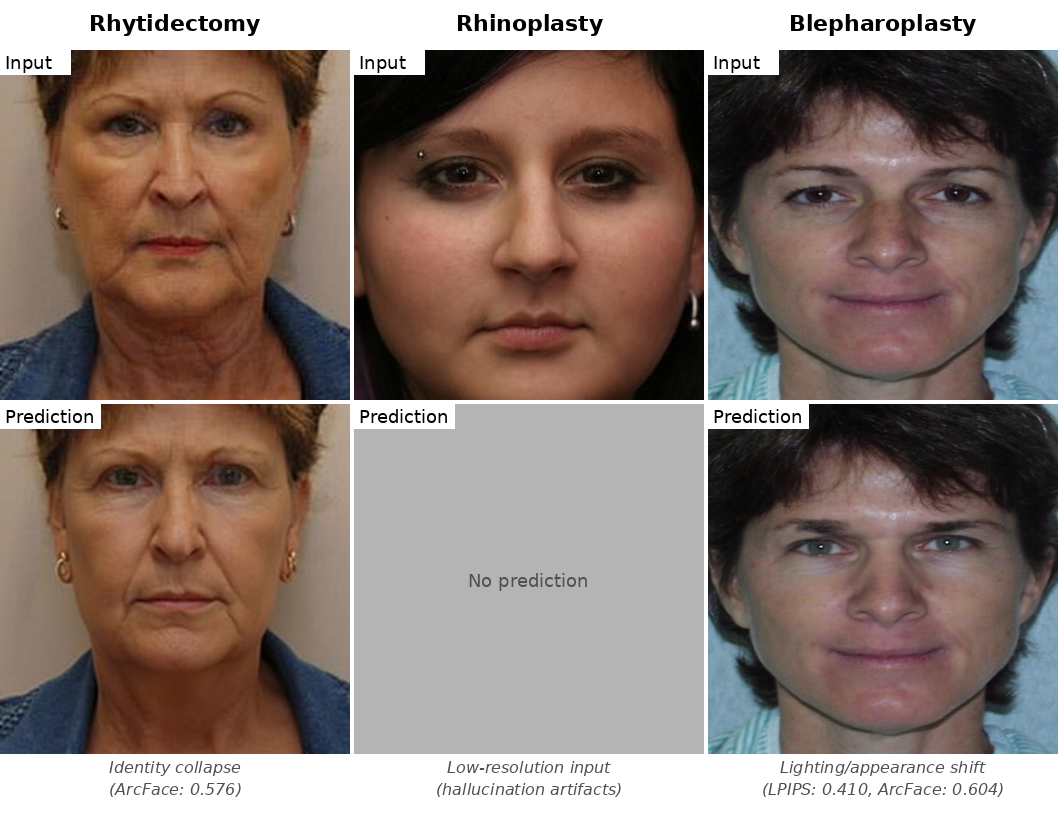
\includegraphics[width=\textwidth]{figures/figS4_failures.png}
\caption{Failure cases: worst-performing test pair per procedure by SSIM.
Top: rhytidectomy identity collapse. Middle: rhinoplasty shape mismatch.
Bottom: blepharoplasty texture artifact. Red metrics indicate SSIM and
LPIPS for each prediction.}
\label{fig:failures}
\end{figure*}

\section{Monk Skin Tone Visualization}

Figure~\ref{fig:skin_tone} shows rhinoplasty predictions across the
Monk Skin Tone (MST) categories present in the HDA test set
(MST~5, 6, and 9). Predictions appear qualitatively consistent across
skin tones, though the limited sample size prevents strong conclusions
about equitable performance.

\begin{figure*}[t]
\centering
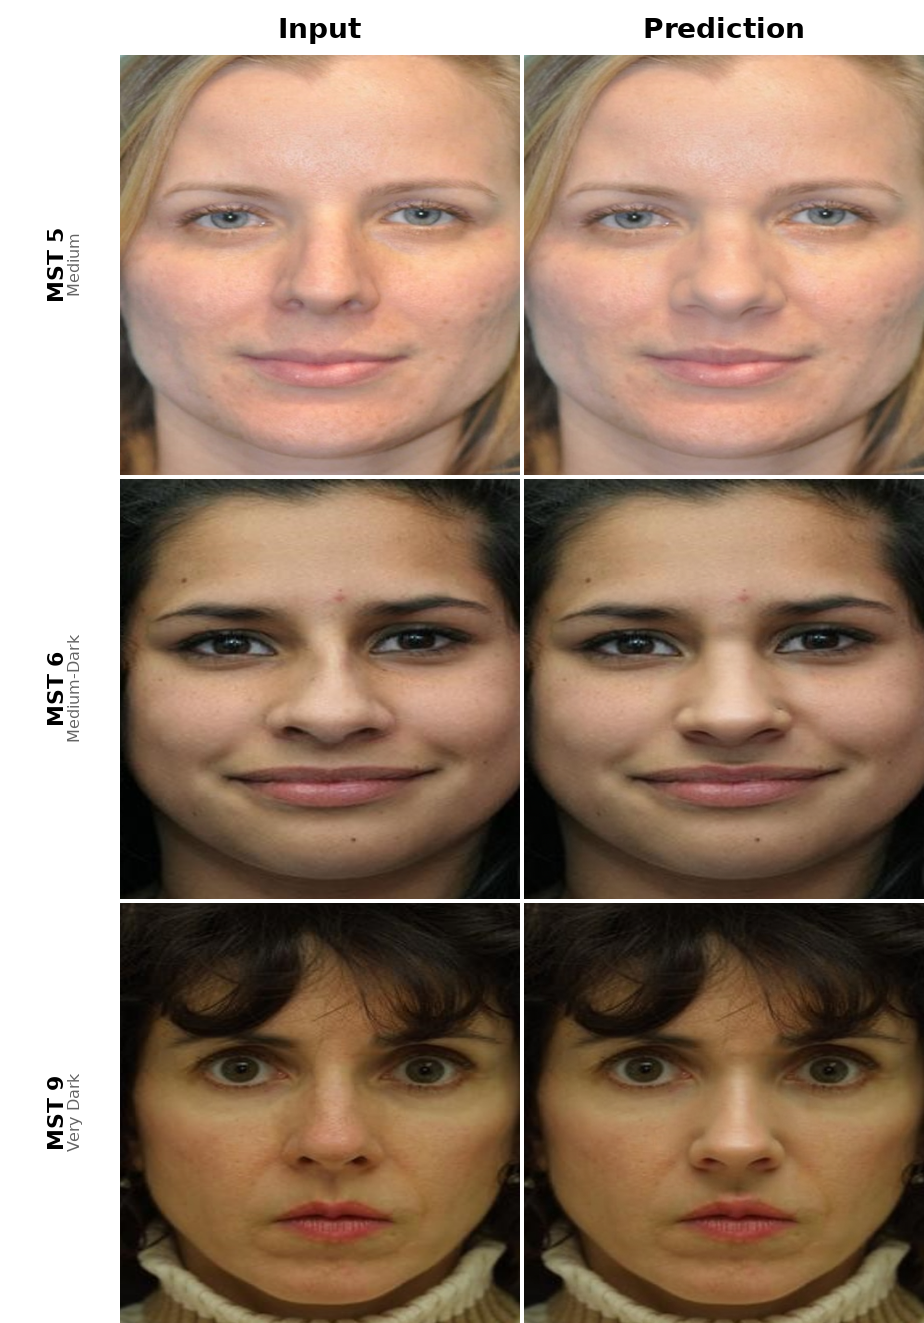
\includegraphics[width=\textwidth]{figures/figS5_skin_tone.png}
\caption{Rhinoplasty predictions across Monk Skin Tone categories
(MST~5, 6, 9). Each row shows input (left) and prediction (right) at
the same pipeline parameters.}
\label{fig:skin_tone}
\end{figure*}

\section{Seed Variation}

Figure~\ref{fig:seed_variation} shows predictions from five different
random seeds for the same rhinoplasty subject (Nose\_27) at identical
pipeline parameters. The visual differences between seeds are subtle but
measurable: ArcFace scores vary by 1 to 3 percentage points across
seeds. The 3-seed sweep selects the output with the highest ArcFace
similarity to the input, providing a modest but consistent improvement
in identity preservation without additional training.

\begin{figure*}[t]
\centering
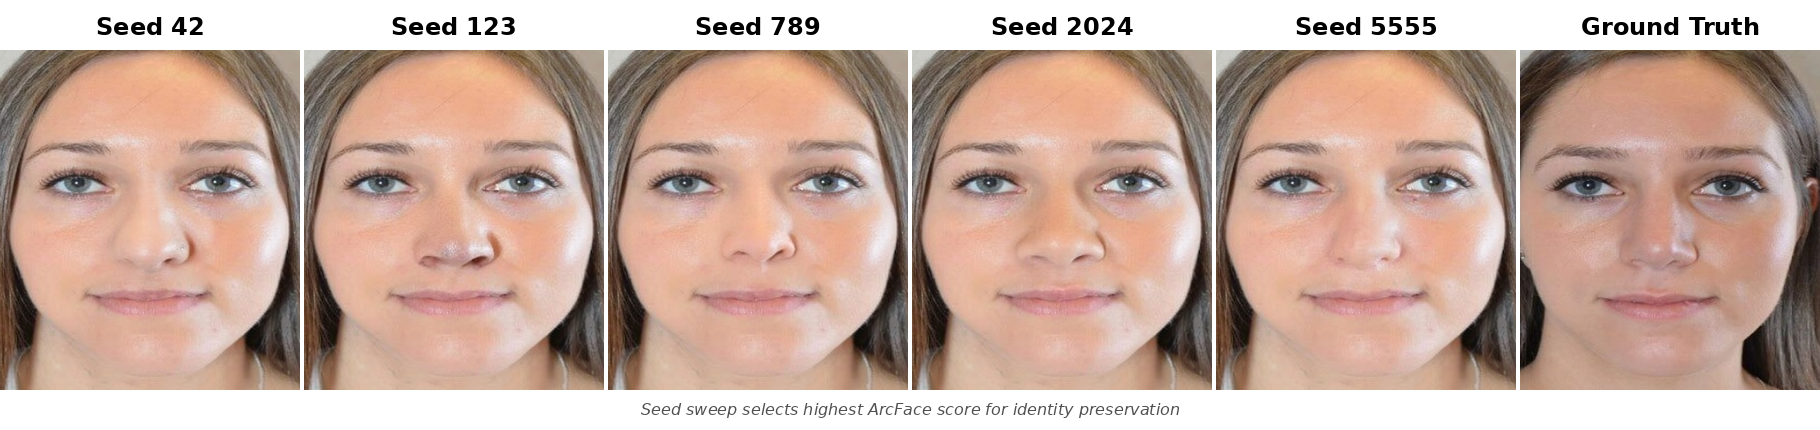
\includegraphics[width=\textwidth]{figures/figS6_seed_variation.png}
\caption{Seed variation for rhinoplasty (Nose\_27). Five different random
seeds produce visually similar but measurably different predictions. The
green border indicates the seed selected by the ArcFace identity gate.}
\label{fig:seed_variation}
\end{figure*}

\end{document}
